\section{Each catalog at equal event counts}
\label{app:pure}

The single-catalog analyses of \S\ref{sec:results:single} confound two things:
what a catalog's redshift prior is worth per event, and the cost of the events
it does not host. To separate them, we drew two further sets of
\PureNevents\ detected events for each realisation of the simulated universe,
one with every host a galaxy and one with every host an AGN, each with
independent measurement noise, and analysed each set against its own
catalog alone, exactly as in \S\ref{sec:results:single} but with nothing
misassigned.

\begin{figure*}[t]
\centering
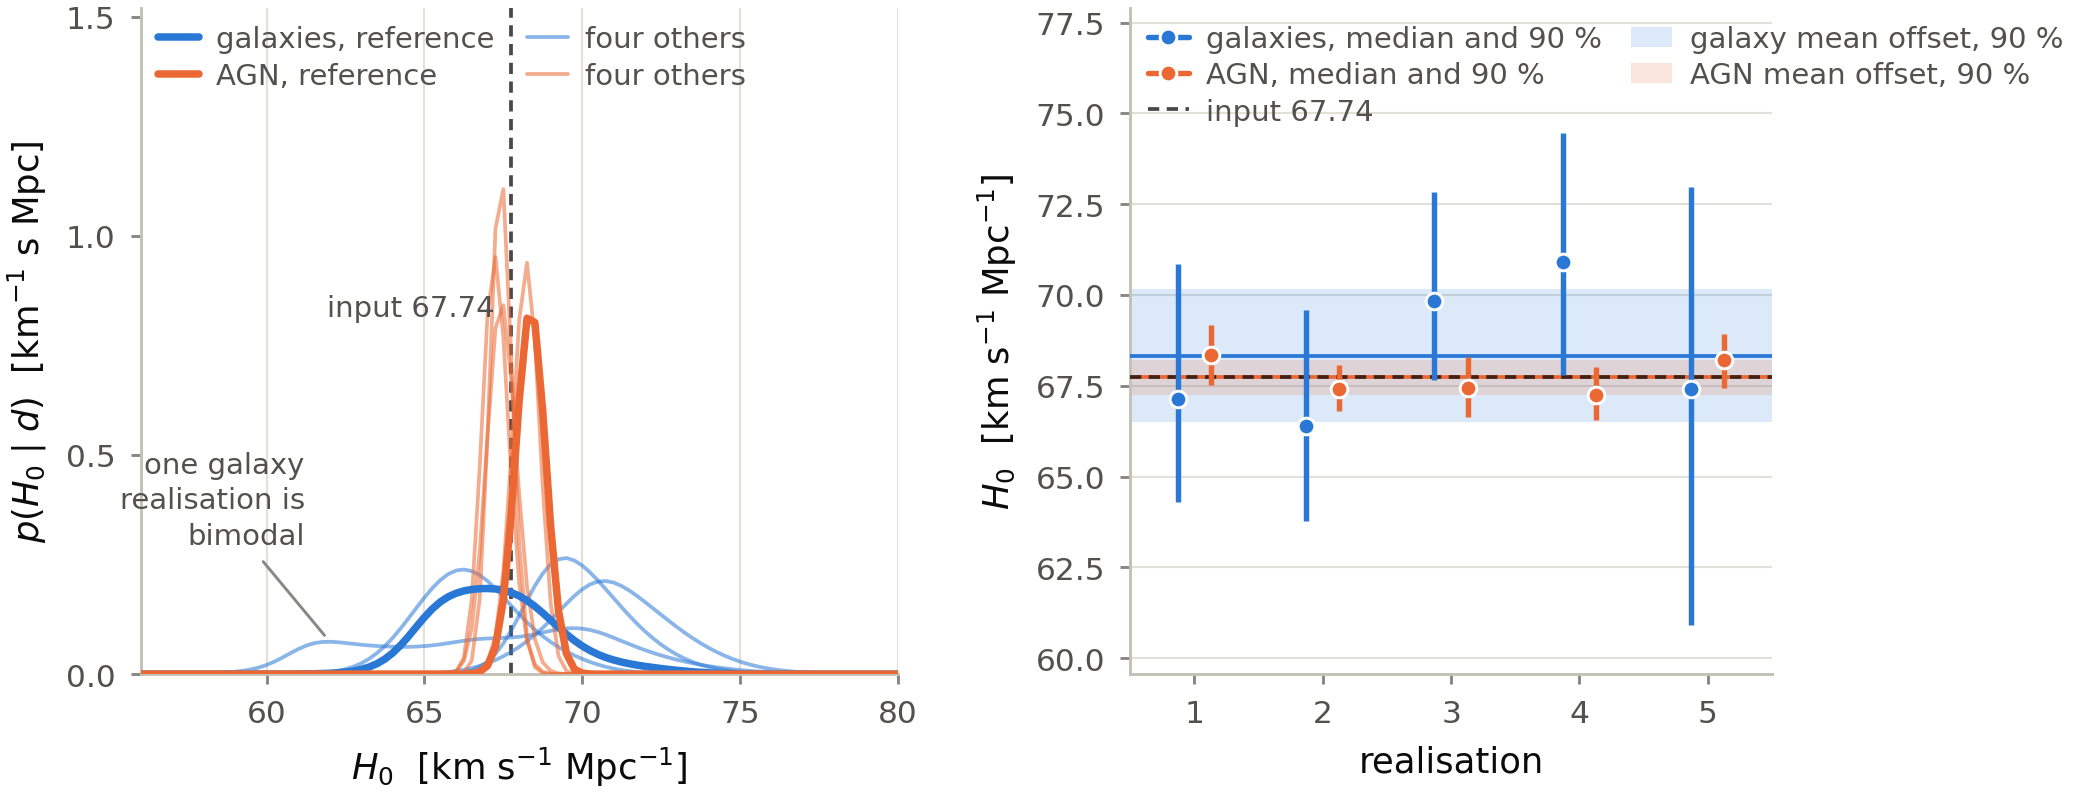
\includegraphics[width=\textwidth]{figures/fig_pure_tracer.pdf}
\caption{What each catalog delivers on events it actually hosts. For every
realisation of the simulated universe, two further sets of \PureNevents\
detected events were drawn on the same catalogs, every host a galaxy
(blue) or every host an AGN (orange), and each set analysed against its
own catalog alone, with \Hz\ the only free parameter. Left: the ten
normalised posterior densities $p(\Hz \mid d)$, in units of
km$^{-1}$\,s\,Mpc, on one shared density axis with no rescaling, and the
input value dashed; the reference realisation is drawn at full strength and
the other four lighter in the same hue, and the \Hz\ axis spans
$[56, 80]$~\kmsmpc, outside which every curve holds less than $10^{-4}$ of
its mass. The bimodal galaxy realisation
(realisation \PureBimodalSeed, second mode at \PureBimodalModeLo~\kmsmpc\ at
\PureBimodalHeight\ of the primary mode at \PureBimodalModeHi) is drawn as it
is. Right: the same ten
measurements as medians with 68\% intervals against the same input line,
the two tracers offset slightly from each other at each realisation for
legibility, with each tracer's five-realisation mean offset and its standard
error as line and band. At equal event count, the catalog one hundred times
sparser is a factor of \PureWidthRatio\ sharper.
\label{fig:pure}}
\end{figure*}

Both catalogs recover the input value. Over the \PureNseeds\ realisations the
mean offsets are $\PureAgnOffset$~\kmsmpc\ from the AGN sets and
$\PureGalOffset$ from the galaxy sets, with the input inside the 90\%
intervals in \PureAgnInNinety\ and \PureGalInNinety\ of \PureNseeds\
realisations (Figure~\ref{fig:pure}); the medians agree with those from the
independent cross-check injection set to at most \PureLaneMaxAgn\ of the
corresponding half-width across all twenty analyses. One galaxy realisation
is bimodal, with a second mode at \PureBimodalModeLo~\kmsmpc\ standing at
\PureBimodalHeight\ of the primary mode at \PureBimodalModeHi, and that
second mode is what widens the galaxy
mean offset's standard error; the cross-check on the same events is
unimodal.

What separates the tracers is the width. At the same event count the AGN
catalog measures the expansion rate with a mean 68\% half-width of
\PureAgnHalfWidth~\kmsmpc\ against the galaxy catalog's \PureGalHalfWidth,
a factor of \PureWidthRatio, stable across realisations (per-realisation
ratio $\PureWidthRatioPerSeed$). A catalog one hundred times sparser is not a
weaker version of the same prior: per event that actually belongs to it, it
is several times stronger, because each event's line of sight holds a handful
of candidate hosts rather than a smooth crowd. This is the per-event
information behind the reading of \S\ref{sec:results:joint}, that the joint
fit gains by letting the AGN-hosted events be anchored by the sparse
catalog.
